\documentclass[a4paper,12pt]{article}

% Pacchetti fondamentali
\usepackage[utf8]{inputenc}
\usepackage[italian]{babel}
% Margini ottimizzati: più larghi ai lati (1cm) e più distribuiti in altezza (1.5cm)
\usepackage[top=1.5cm, bottom=1.5cm, left=1cm, right=1cm]{geometry} 
\usepackage{graphicx} 
\usepackage{nopageno} 
\usepackage{xcolor}
\usepackage{amsmath, amssymb} 
\usepackage{fontawesome5} 
\usepackage{tcolorbox} 

% Definizione dei colori personalizzati (Tema Umanistico)
\definecolor{maincolor}{RGB}{128, 0, 32} % Un elegante bordeaux/rosso pompeiano
\definecolor{accent}{RGB}{218, 165, 32} % Un color oro per i dettagli
\definecolor{lightgray}{RGB}{245, 245, 245}

\begin{document}

% --- INTESTAZIONE COLORATA ---
\begin{center}
    {\Huge \textbf{\faLandmark\ MATERIE CLASSICHE E UMANISTICHE}}\\[0.3cm]
    {\Large \textit{Latino, Greco, Italiano, Storia e Geografia}}
\end{center}
\vspace{0.4cm} 

% --- CORPO CENTRALE DIVISO IN DUE ---
\noindent
\begin{minipage}[t]{0.63\textwidth} 
    \vspace{0pt} % <-- TRUCCO: Forza l'allineamento in alto con l'altra minipage
    
    \textcolor{maincolor}{\Large \textbf{\faUserGraduate\ Chi sono}}\\[0.2cm]
    Mi chiamo \textbf{Federica}. Sono laureata con \textbf{110 e Lode} in \textbf{Filologia, Letterature e Storia dell'Antichità} (Laurea Magistrale) e ho una formazione Triennale in Lettere Classiche. Durante il mio percorso accademico ho approfondito la ricerca filologica, partecipando anche come relatrice a conferenze universitarie sulla tradizione agiografica di Santa Cristina.\\
    Ho un'esperienza consolidata nell'insegnamento privato, specialmente nell'affiancamento di studenti del \textbf{Liceo Classico}. \\\textbf{Il mio obiettivo} non è fornirti la traduzione pronta da ricopiare, ma insegnarti un metodo di indagine logico e rigoroso per affrontare i testi antichi e la letteratura con sicurezza e autonomia.\\[0.4cm]
    
    \textcolor{maincolor}{\Large \textbf{\faChalkboardTeacher\ Cosa offro}}\\[0.2cm]
    \begin{itemize}
        \setlength{\itemsep}{0.25cm} 
        \item[\textcolor{accent}{\faCheckCircle}] \textbf{Licei:} Supporto specialistico per le versioni di Greco e Latino, recupero delle basi grammaticali e approfondimento della letteratura.
        \item[\textcolor{accent}{\faCheckCircle}] \textbf{Medie e Superiori:} Ripetizioni di Italiano, Storia, Geografia e materie umanistiche in generale per costruire un metodo di studio efficace.
        \item[\textcolor{accent}{\faCheckCircle}] \textbf{Preparazione Mirata:} Creiamo insieme un percorso su misura per superare verifiche scritte, interrogazioni o \textbf{recupero debiti} senza ansia.
        \item[\textcolor{accent}{\faCheckCircle}] \textbf{Zero Perdite di Tempo:} Ti chiedo di indicarmi gli argomenti prima della lezione. In questo modo preparo schemi, vocabolario ed esercizi per sfruttare al 100\% il nostro tempo.
        \item[\textcolor{accent}{\faCheckCircle}] \textbf{Online o in Presenza:} Flessibilità totale. Lezioni a distanza tramite strumenti interattivi o in presenza se residenti in zona.
    \end{itemize}\vspace{0.4cm}
    
    \textcolor{maincolor}{\Large \textbf{\faAddressCard\ Contatti}}\\[0.2cm]
    \faPhoneSquare\ Telefono / WhatsApp: \textbf{389\,0179057}\\
    \faEnvelope\ Email: \textbf{federicafavagrossa@gmail.com}
    
\end{minipage}%
\hfill
\begin{minipage}[t]{0.34\textwidth}
    \vspace{0pt} % <-- TRUCCO: Si allinea esattamente alla prima riga di "Chi sono"

    % --- IMMAGINE CENTRALE ---
    \begin{center}
        % Sostituisci "immagine_classica.jpg" con il nome della tua immagine
        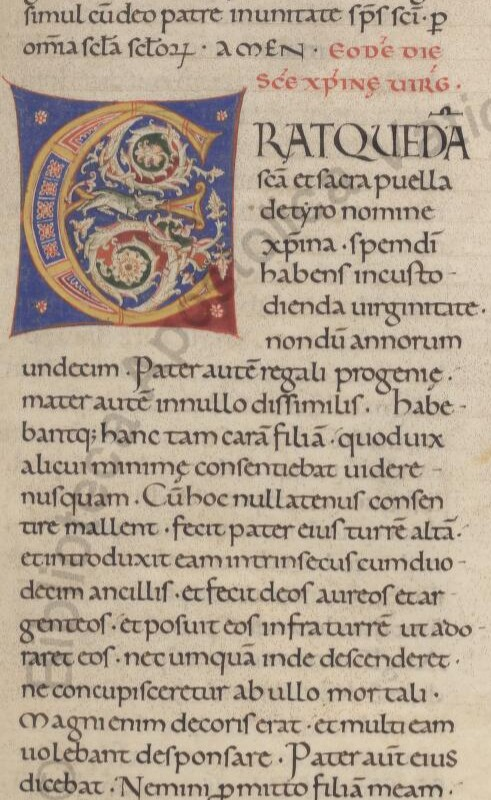
\includegraphics[width=0.82\textwidth, keepaspectratio]{immagine_classica.jpg}\\
        \vspace{0.15cm}
        \small\textit{Manoscritto Barb.lat.586 del XII-XIII secolo.}
        \vspace{0.4cm} 
    \end{center}

    % --- RIQUADRO SPECIALE AGOSTO ---
    \begin{tcolorbox}[colback=lightgray, colframe=maincolor, arc=2mm, title=\faSun\ \textit{Speciale Recupero Debiti}, left=4pt, right=4pt, top=5pt, bottom=5pt, boxsep=2pt]
        \centering
        \small \textbf{Disponibilità ad Agosto}\\[0.2cm]
        \textit{Hai un esame di riparazione a settembre?}\\[0.2cm]
        Sono disponibile nel mese di \textbf{agosto} per percorsi di studio intensivi e mirati. Costruiamo un piano di recupero per arrivare all'esame sicuri e preparati!\\[0.1cm]
    \end{tcolorbox}
    
    \vspace{0.4cm}
    
    \begin{center}
        % Spazio per QR Code 
        
\includegraphics[width=3.9cm]{qr.jpeg}\\[0.15cm]
        \small \faLinkedin\ \textit{Inquadra per il mio profilo!}
    \end{center}
\end{minipage}

\end{document}
